\documentclass[conference]{IEEEtran}

\usepackage{cite}
\usepackage{amsmath,amssymb,amsfonts}
\usepackage{algorithmic}
\usepackage{graphicx}
\usepackage{textcomp}
\usepackage{xcolor}

\def\BibTeX{{\rm B\kern-.05em{\sc i\kern-.025em b}\kern-.08em
    T\kern-.1667em\lower.7ex\hbox{E}\kern-.125emX}}

\begin{document}

\title{Convolutional Neural Networks for the Prediction of ASD and 
       Biomarker Identification}

\author{
    \IEEEauthorblockN{Tony Kabilan Okeke}
    \IEEEauthorblockA{\textit{School of Biomedical Engineering} \\
    \textit{Drexel University}\\
    Philadelphia, PA \\
    tko35@drexel.edu}
}

\maketitle

\begin{abstract}
    The abstract will go here.
\end{abstract}

\begin{IEEEkeywords}
    connectomics, CNN, biomarker, autism, ASD
\end{IEEEkeywords}

% ----------------------------------------------------------------------------------------

\section{Introduction}

Autism Spectrum Disorder (ASD) is a neurodevelopmental disorder that is characterized by 
social and communicationdeficits as well as restricted, repetitive behaviors. Early 
diagnosis and intervention are critical for improvinglong-term outcomes; however, the 
current gold standard assessment tools are limited in their ability to accurately and 
efficiently diagnose ASD, particularly in young children. Typically, ASD diagnoses are 
based on behavioral criteria, but there is growing interest in the identification of 
objective biomarkers to aid in the diagnoses \cite{Shen.2019}. Biomarkers are measurable 
characteristics that can be used to indicate the presence or severity of a disease. In the 
case of ASD, biomarkers could be used to improve and validate diagnoses, especially in 
young children, and potentially before the emergence of symptoms.

Due to advancements in multimodal neuroimaging in recent years, neuroscience has gained 
unprecedented opportunities to interrogate the living human brain at multiple scales in 
both health and disease \cite{Hong.2019}, and these advancements have been especially 
useful in the study of neurodevelopmental disorders \cite{Nunes.2019}.

Several studies have been conducted to examine changes in functional connectivity in 
individuals with ASD relative to typically developing controls \cite{Lau.2019, Williams.2013}. 
However, less is known about changes in structural connectivity in individuals with ASD. 
By capitalizing on diffusion-weighted magnetic resonance imaging (dMRI), previous studies 
were able to identify abnormalities in the connectivity strength of several inter-regional 
fiber pathways in individuals with ASD \cite{dAlBbis.2018}. Despite the identification of 
these abnormalities, the diagnosis of ASD based on brain imaging remains a challenge. 
One reason for this challenge is that the abnormalities associated with ASD are often 
subtle and are often difficult to detect. This calls for the application of sophisticated 
computational methods to aid in the diagnoses.

In recent years, there has been an explosion of interest in the potential of machine 
learning to revolutionize different aspects of neuroscience \cite{Abos.2017,Vogt.2018}. 
However, given the complex and high-dimensional nature of connectomes, traditional 
machine learning approaches are not well-suited for connectome classification problems. 
Recent advances in deep learning, specifically Convolutional Neural Networks (CNNs), have 
shown promise in the prediction of clinical neurodevelopmental outcomes from brain 
networks (connectomes). For example, \textit{BrainNetCNN} was developed for the 
prediction of cognitive and motor scores from the connectomes of infants born preterm 
\cite{Kawahara.2017}.

% ----------------------------------------------------------------------------------------

\section{Materials and Methods}

    \subsection{Materials}

    In this paper, we seek to develop and validate a deep-learning based connectome 
    classification model to distinguish between the structural connectomes of individuals 
    with ASD and typically developing controls. By utilizing a combination of different 
    feature selection techniques, we also hope to identify potential biomarkers that 
    could aid in the diagnosis of ASD. ``Fig.~\ref{project-schematic}'' provides an 
    outline of the project. 

    For this purpose we will utilize a collection dMRI-derived structural connectomes 
    from a large collection of individuals with ASD, as well as typically developing 
    controls obtained from collaborators at the University of Pennsylvania. This data 
    will be utilized for the training and validation of the model.

    \begin{figure}[ht]
        \vskip 0.2in
        \begin{center}
            \centerline{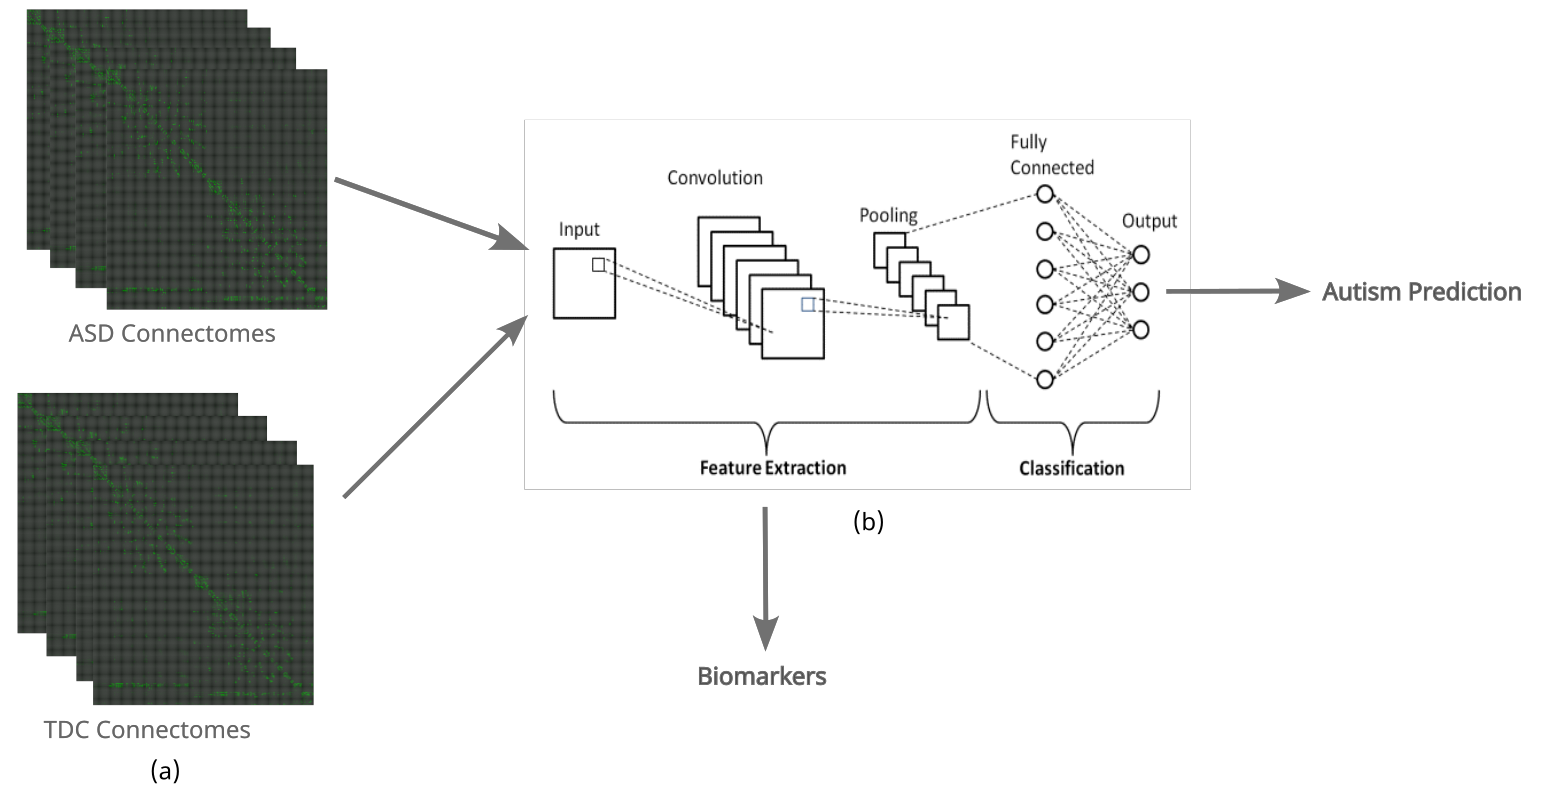
\includegraphics[width=\columnwidth]{../img/project_schematic_v1.png}}
            \caption{
                Overview of autism prediction and biomarker identification using a 
                Convolutional Neural Network based classifier. (a) (top) Structural 
                connectomes of patients with Autism Spectrum Disorder. (bottom) Structural 
                connectomes of Typically Developing Controls. (b) Schematic diagram for 
                convolutional neural network.
            }
            \label{project-schematic}
        \end{center}
        \vskip -0.2in
    \end{figure}

% ----------------------------------------------------------------------------------------

\begin{thebibliography}{00}
    \bibitem{Abos.2017} {Abos, A., Baggio, H., Segura, B., Garcia-Diaz, A., Compta, Y., Marti, M., Valldeoriola, F., \& Junqué, C. (2017). Discriminating cognitive status in Parkinson’s disease through functional connectomics and machine learning. Scientific reports, 7(1), 1–-13.}
    \bibitem{dAlBbis.2018} {d`Albis, M.A., Guevara, P., Guevara, M., Laidi, C., Boisgontier, J., Sarrazin, S., Duclap, D., Delorme, R., Bolognani, F., Czech, C., \& others (2018). Local structural connectivity is associated with social cognition in autism spectrum disorder. Brain, 141(12), 3472–-3481.}
    \bibitem{Craddock.2013} {Craddock, R., Jbabdi, S., Yan, C.G., Vogelstein, J., Castellanos, F., Di Martino, A., Kelly, C., Heberlein, K., Colcombe, S., \& Milham, M. (2013). Imaging human connectomes at the macroscale. Nature methods, 10(6), 524–-539.}
    \bibitem{Hong.2019} {Hong, S.J., Wael, R., Bethlehem, R., Lariviere, S., Paquola, C., Valk, S., Milham, M., Di Martino, A., Margulies, D., Smallwood, J., \& others (2019). Atypical functional connectome hierarchy in autism. Nature communications, 10(1), 1–-13.}
    \bibitem{Kawahara.2017} {Kawahara, J., Brown, C., Miller, S., Booth, B., Chau, V., Grunau, R., Zwicker, J., \& Hamarneh, G. (2017). BrainNetCNN: Convolutional neural networks for brain networks; towards predicting neurodevelopment. NeuroImage, 146, 1038-–1049.}
    \bibitem{Lau.2019} {Lau, W., Leung, M.K., \& Lau, B. (2019). Resting-state abnormalities in autism spectrum disorders: a meta-analysis. Scientific reports, 9(1), 1–-8.}
    \bibitem{Nunes.2019} {Nunes, A., Peatfield, N., Vakorin, V., \& Doesburg, S. (2019). Idiosyncratic organization of cortical networks in autism spectrum disorder. Neuroimage, 190, 182-–190.}
    \bibitem{Osmanlioglu.2019} {Osmanlioglu, Y., Tunc, B., Parker, D., Elliott, M., Baum, G., Ciric, R., Satterthwaite, T., Gur, R., Gur, R., \& Verma, R. (2019). System-level matching of structural and functional connectomes in the human brain. NeuroImage, 199, 93–-104.}
    \bibitem{Rubinov.2019} {Rubinov, M., \& Sporns, O. (2010). Complex network measures of brain connectivity: uses and interpretations. Neuroimage, 52(3), 1059-–1069.}
    \bibitem{Salari.2020} {Sherkatghanad, Z., Akhondzadeh, M., Salari, S., Zomorodi-Moghadam, M., Abdar, M., Acharya, U., Khosrowabadi, R., \& Salari, V. (2020). Automated detection of autism spectrum disorder using a convolutional neural network. Frontiers in neuroscience, 13, 1325.}
    \bibitem{Shen.2019} {Shen, L., Zhao, Y., Zhang, H., Feng, C., Gao, Y., Zhao, D., Xia, S., Hong, Q., Iqbal, J., Liu, X., \& others (2019). Advances in biomarker studies in autism spectrum disorders. Reviews on Biomarker Studies in Psychiatric and Neurodegenerative Disorders, 207–-233.}
    \bibitem{Tunc.2021} {Tunç, B., Pandey, J., St. John, T., Meera, S., Maldarelli, J., Zwaigenbaum, L., Hazlett, H., Dager, S., Botteron, K., Girault, J., \& others (2021). Diagnostic shifts in autism spectrum disorder can be linked to the fuzzy nature of the diagnostic boundary: a data-driven approach. Journal of Child Psychology and Psychiatry, 62(10), 1236–-1245.}
    \bibitem{Vogt.2018} {Vogt, N. (2018). Machine learning in neuroscience. Nature Methods, 15(1), 33–-33.}    
    \bibitem{Williams.2013} {Williams, D., Cherkassky, V., Mason, R., Keller, T., Minshew, N., \& Just, M. (2013). Brain function differences in language processing in children and adults with autism. Autism Research, 6(4), 288–-302.}

\end{thebibliography}

\end{document}
